%%=============================================================================
%% Inleiding
%%=============================================================================

\chapter{\IfLanguageName{dutch}{Functionele Omschrijving TAC2.0}{Functional Description TAC2.0}}
\label{ch:functionele-omschrijving}

Het checkoutsysteem van Colruyt Group, \textbf{FVS} (``filiaalverkoopsysteem''), bestaat uit een verscheidenheid aan individuele componenten en is verwoven met zo goed als elk domein binnen de firma — gaande van marketing en customer management tot herbevoorrading en accountancy. Een grondige kennis van dit systeem, en in het bijzonder de werking van de kassa vanuit het perspectief van de kassabediende, is dan ook onontbeerlijk voor dit onderzoek.

\section{Hardware}

Kassabedienden en verkopers in de filialen van Colruyt, Colruyt France, OKay, OKay City, Bio-Planet, Dreamland, Dreambaby, en Colruyt Group Spar zijn kennen het checkoutsysteem vooral als ``de \textbf{TAC}''. ``TAC'' komt van het Engelse woord ``tactile'' en verwijst naar het feit dat het scherm voornamelijk bediend wordt door er op te tikken met de vingers.

\subsection{Opstellingen}

Er zijn grosso modo 2 verschillende opstellingen:

\begin{enumerate}
     \item \textbf{Gescheiden}. Het registreren en afhandelen van klantenaankopen gebeurt in twee stappen. In de eerste stap worden zijn aankopen geregistreerd, alsook worden eventuele kortingsbonnen en klantenkaarten aan de rekening toegevoegd. Het TAC-scherm dat daarvoor gebruikt wordt, staat bekend als de \textbf{CTAC} ('C' voor ``controle''). De betaling vindt vervolgens plaats aan een tweede scherm, gekend als de \textbf{PTAC} ('P' voor ``payment''). De klanten van Colruyt, OKay en Bio-Planet zijn vertrouwd met deze opstelling.
     \item \textbf{Gecombineerd}. Het is ook mogelijk om het volledige kassaproces aan één TAC-scherm af te ronden, zoals in OKay City, Dreamland, Dreambaby en Colruyt Group Spar winkels gebeurt. In dat geval wisselt het systeem tussen het registratiescherm en het betaalscherm, afhankelijk van de gebruikssituatie. Er zijn meerdere opstellingen die aan dit profiel voldoen, met name de \textbf{MTAC} ('M' voor ``multi'') en de \textbf{KTAC} ('K' voor ``\emph{k}ombinatie''). Hun onderlinge verschillen worden niet verder behandeld.
\end{enumerate}

\begin{figure}%
    \centering
    \subfloat{{\includegraphics[width=6cm]{img/func-omsch/CTAC-OKay-Overzetten.jpg} }}%
    \qquad
    \subfloat{{\includegraphics[width=6cm]{img/func-omsch/PTAC-OKay.jpg} }}%
    \caption{Links: CTAC opstelling, rechts: PTAC opstelling — beide in het OKay opleidingslokaal op de Wilgenveld site in Halle.}%
    \label{fig:ctac-ptac-okay}%
\end{figure}

\subsection{Randapparaten}

Een TAC opstelling is voorzien van enkele randapparaten (``peripherals''), afhankelijk van het soort TAC opstelling dat gebruikt wordt:

\begin{itemize}
    \item \textbf{3D barcodelezer} — wordt gebruikt voor het inlezen van artikelbarcodes, pakketten, kortingsbonnen en klantenkaarten. De barcodelezer wordt niet voorzien aan een PTAC opstelling.
    \item \textbf{Tafelscanner} — alternatief voor de barcodelezer dat in het kassameubel van Dreamland, Dreambaby en sommige Spar winkelformules ingebouwd wordt.
    \item \textbf{Kaartlezer} — ingebouwd in de TAC hardware. Laat toe klantenkaarten in te lezen aan de hand van hun magneetstrook. Dit apparaat wordt zelden gebruikt, maar laat wel toe om klantenkaarten met een betaalfunctie in te lezen aan de PTAC.
    \item \textbf{Weegschaal} — wordt niet voorzien aan een PTAC opstelling of in de \emph{non-food} winkelformules (Dreamland en Dreambaby).
    \item \textbf{Klantendisplay} — geeft de klant informatie over de geregistreerde items aan de PTAC in Colruyt, OKay en Bio-Planet. In Spar winkels geeft het klantendisplay ook informatie over het betalingsverloop.
    \item \textbf{Lamp} — een Colruyt CTAC opstelling gebruikt een hangende lamp boven de winkelkar als visuele feedback op artikelregistraties.
    \item \textbf{Betaalterminal} — laat betalingen met debet-, krediet-, en maaltijdcheque kaarten toe. Klanten die met een interne betaalkaart (Xtrakaart met betaalfunctie, Colruytkaart) betalen, gebruiken de terminal ook om hun geheime code in te tikken.
    \item \textbf{Geldlade} — PTAC en MTAC/KTAC configuraties sturen ook de geldlade aan, die ze kunnen openen en wiens sluiting ze ook kunnen detecteren.
\end{itemize}

\section{Systeemarchitectuur}

De high level systeemarchitectuur van FVS wordt geschetst in figuur \ref{fig:FVSHighLevel}.

\begin{figure}[h!]
    \centering
    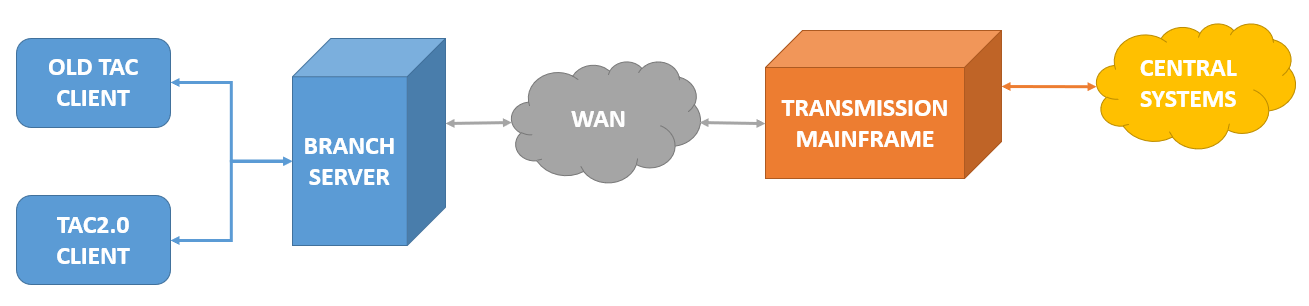
\includegraphics[scale=0.35]{img/func-omsch/DiagramHighLevel.PNG}
    \caption{High level view van FVS, het checkoutsysteem van Colruyt Group.}
    \label{fig:FVSHighLevel}
\end{figure}

Elk filiaal beschikt over één \textbf{filiaalserver} die met de centrale systemen communiceert. Afhankelijk van de richting van die communicatie spreekt men binnen Colruyt Group over ``mutaties'', ``transmissies'' of over ``online transacties''.

\begin{itemize}
    \item Een \textbf{mutatie} is het versturen van data van een centraal systeem naar één specifieke filiaalserver, waaronder artikeldata (het assortiment en prijzen), promoties, en de gegevens van klantenkaarten. Dit kunnen kreaties [sic], wijzigingen, of eliminaties zijn.
    \item Een \textbf{transmissie} is de omgekeerde beweging en gaat voornamelijk over verkoopsgegevens (kastickets, voorraadwijzigingen etc.). Mutaties en transmissies gebeuren voornamelijk 's nachts, hoewel sommige soorten (dringende correcties) ook tijdens de operationele uren gebeuren.
    \item \textbf{Online transacties} zijn ten slotte (meestal synchrone) web services voor tijdgevoelige communicatie, zoals het controleren van klantenkaarten en het afhandelen van betalingen met de Xtra of Colruyt kaart.
\end{itemize}

De FVS filiaalserver communiceert nooit rechtstreeks met de centrale systemen; de \textbf{transmissie mainframe} neemt de verantwoordelijkheid voor het valideren en formatteren van mutaties, het initiëren en afhandelen van transmisies, en biedt aan FVS een service (\emph{ProcessBranchRequest}) aan voor online transacties.

Figuur \ref{fig:FVSDetail} modelleert de filiaalserver en zijn onmiddellijke context.

\begin{figure}[h!]
    \centering
    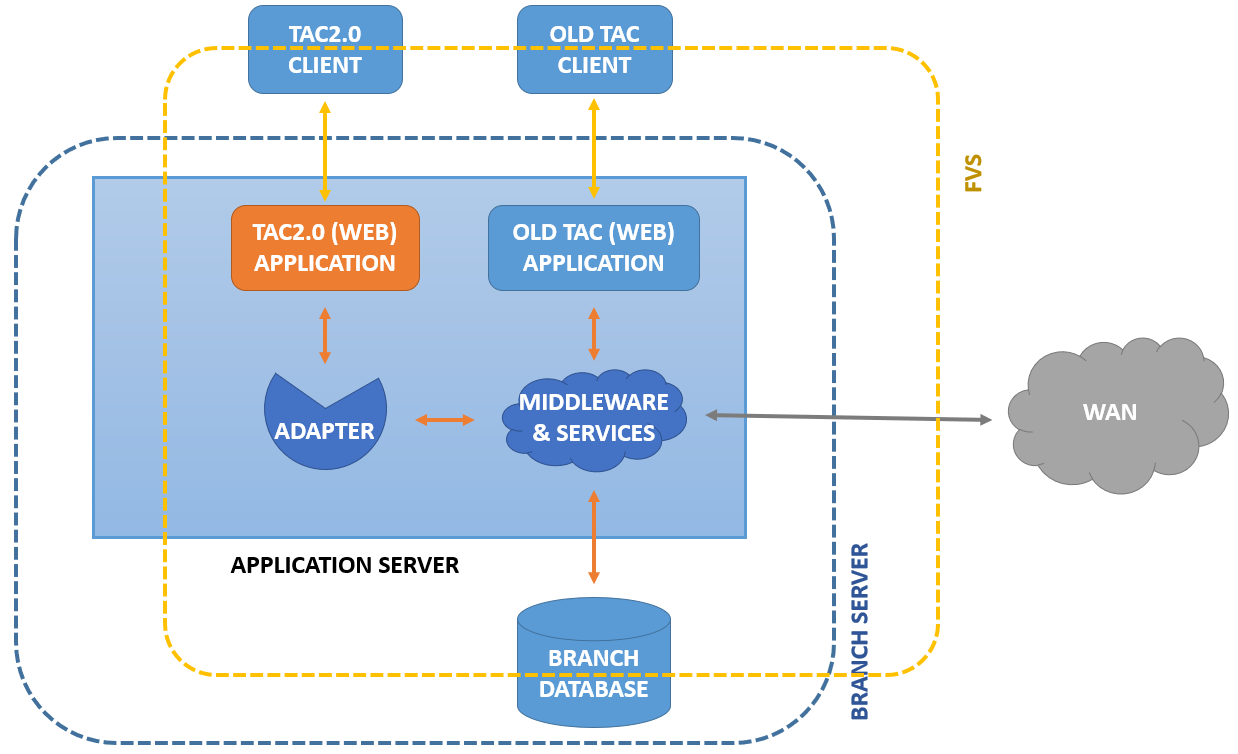
\includegraphics[scale=0.35]{img/func-omsch/DiagramLowerLevel.PNG}
    \caption{Gedetailleerd overzicht van de architectuur van de filiaalservers die Colruyt Group gebruikt.}
    \label{fig:FVSDetail}
\end{figure}

De frontend van het kassasysteem, zowel de huidige versie als de toekomstige TAC2.0 versie, is een webapplicatie die op de (lokale) filiaalserver draait. De TAC client is een ``lege doos'' die bij opstart zijn basisconfiguratie ontvangt van de cradle waar deze op aangesloten zit, en vervolgens een image van zijn stripped-down besturingssysteem download van de filiaalserver. Dit laat toe om TAC schermen te wisselen zonder manuele configuratiewijzigingen.

De TAC client navigeert, middels een browser (Chromium in het geval van TAC2.0), naar het adres van deze webapplicatie bij de opstart van de client. Deze webapplicatie wordt gehost op een Websphere application server die runt op de filiaalserver. Naast de webapplicatie zelf, runnen een reeks middleware applicaties en services eveneens op de virtuele applicatie server.

Deze middleware en services worden aangeroepen door de TAC frontend om diverse taken te voltooien, waaronder het registreren van transacties, het afhandelen van een elektronische betaling, en het activeren van geschenkkaarten. De TAC2.0 webapplicatie gebruikt op het moment van schrijven een adapter om deze middleware en services te kunnen gebruiken, hoewel die laatsten op termijn ook herschreven zullen worden.

Tot slot runt de filiaalserver ook een databank, die voornamelijk gebruikt wordt door het FVS systeem. Zoals figuur \ref{fig:FVSDetail} suggereert, zijn er nog andere toepassingen die gebruik maken van de applicatie server en de databank die zich op de filiaalserver bevinden. Dit zijn voornamelijk winkelapplicaties die hier niet verder besproken worden.

\section{Gebruikersinterface}

De gebruikersinterface van TAC2.0 werd ontworpen met continuïteit als het belangrijkste criterium. Om die reden is de gebruikersinterface en bijhorende user experience design grotendeels dezelfde als die van de oude TAC.

\begin{figure}%
    \centering
    \subfloat{{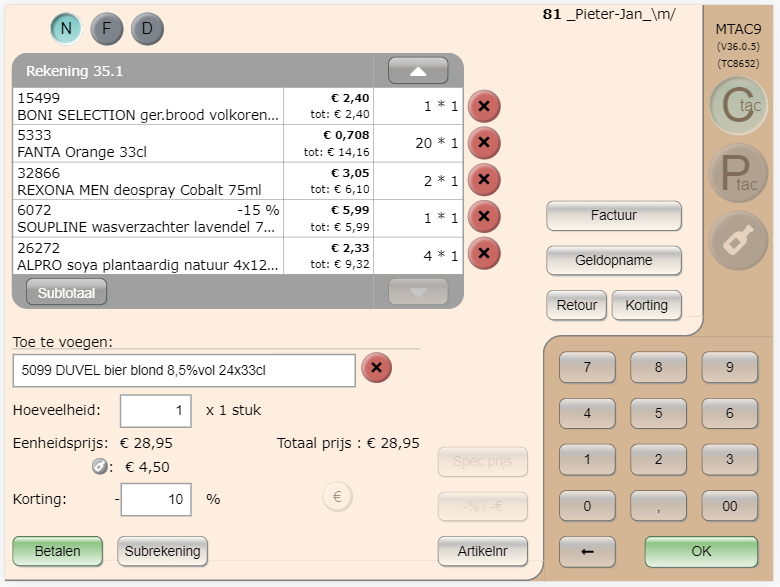
\includegraphics[width=6cm]{img/func-omsch/CLP-CTAC-ArtikelMetLeeggoedEnKorting.PNG} }}%
    \qquad
    \subfloat{{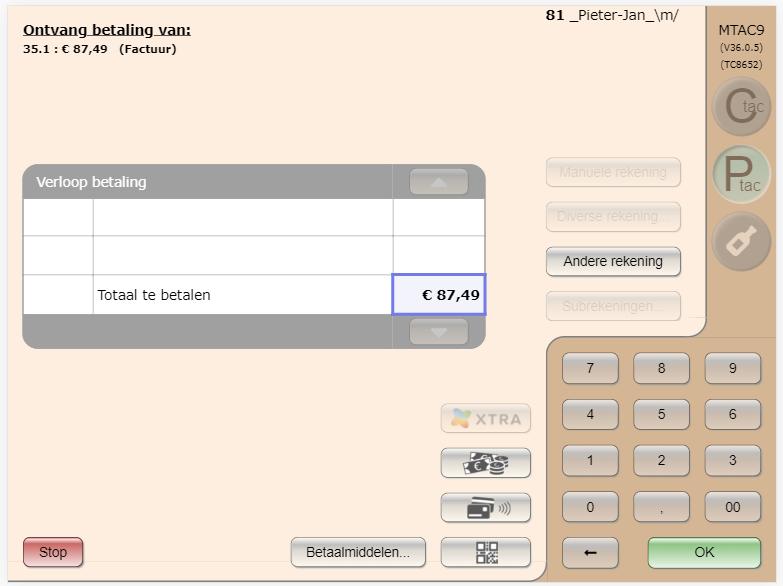
\includegraphics[width=6cm]{img/func-omsch/CLP-PTAC-BeginBetalen.PNG} }}%
    \caption{Links: CTAC interface nadat een artikel met leeggoedwaarde werd toegevoegd en een percentkorting werd toegekend. Rechts: PTAC interface aan het begin van het betalingsproces. \scriptsize Copyright~\copyright~Colruyt Group Services nv}%
    \label{fig:ctac-ptac-ui}%
\end{figure}

Figuur \ref{fig:ctac-ptac-ui} toont de belangrijkste schermen van de TAC2.0 frontend: het artikelenoverzicht op de CTAC en het betalingsoverzicht op de PTAC. Merk op dat deze specifieke beelden afkomstig zijn van een MTAC opstelling; een aparte CTAC en PTAC opstelling hebben dezelfde layout, m.u.v. kleine verschillen tussen de retailformules onderling.

\subsection{CTAC}

Figuur \ref{fig:Ctac-Aangeduid} toont de verschillende onderdelen van het basisscherm van de CTAC opstelling:

\begin{enumerate}
    \item De \emph{TransactionListComponent} \textbf{(1)} toont een overzicht van de geregistreerde transacties voor de huidige rekening, waaronder artikelen — met hun eenheidsprijs, hoeveelheid (of gewicht), totale prijs, en eventuele kortingen — klantenkaarten, kortingsbonnen, geldopnames etc. Transacties kunnen geannuleerd worden met de rode knop.
    \item De \emph{ArticleNumberComponent} \textbf{(2)} laat toe artikelen te registreren, aan de hand van een barcode of door het intern artikelnummer manueel in te tikken gebruik makende van het numeriek toestenbord. Hier kan ook de hoeveelheid (of het gewicht) aangepast worden, kan een speciale prijs toegekend worden, en kan een korting (procentueel of als bedrag) toegekend worden.
    \item Het numeriek toetsenbord \textbf{(3)} is deel van de \emph{XTacStartUpComponent} en dus altijd beschikbaar, ook op het inlogscherm.
    \item De \emph{SalesActionButtonsComponent} \textbf{(4)} geeft verschillende opties, afhankelijk van het winkeltype. In Colruyt hebben we de mogelijkheid factuurgegevens toe te voegen, een geldopname in te geven, een artikel als retour te registreren, of een globale korting toe te kennen.
    \item De \emph{LanguageButtonsComponent} \textbf{(5)} geeft aan in welke taal het kasticket van de klant geprint zal worden. Elke winkel heeft een standaardtaal, die manueel of middels een klantenkaart gewijzigd kan worden.
    \item De \emph{SaleButtonsComponent} \textbf{(6)} bevat de knoppen om de rekening af te sluiten of om een subrekening aan te maken. Op een CTAC opstelling zal de ``betalen'' knop zorgen voor de totalisatie van de rekening, waarna de operator uitgelogd wordt en de rekening kan oproepen op een PTAC toestel. Op een MTAC opstelling krijgt de gebruiker onmiddellijk het betaalscherm te zien. Subrekeningen maken het mogelijk een kar te splitsen — en dus aparte kastickets te krijgen — maar kunnen meestal wel samen betaald worden.
    \item De overige componenten rechtsboven \textbf{(7)} geven informatie over de aangelogde operator (operatornummer \& roepnaam), de toestelconfiguratie, en de softwareversie.
\end{enumerate}

\begin{figure}[h!]
    \centering
    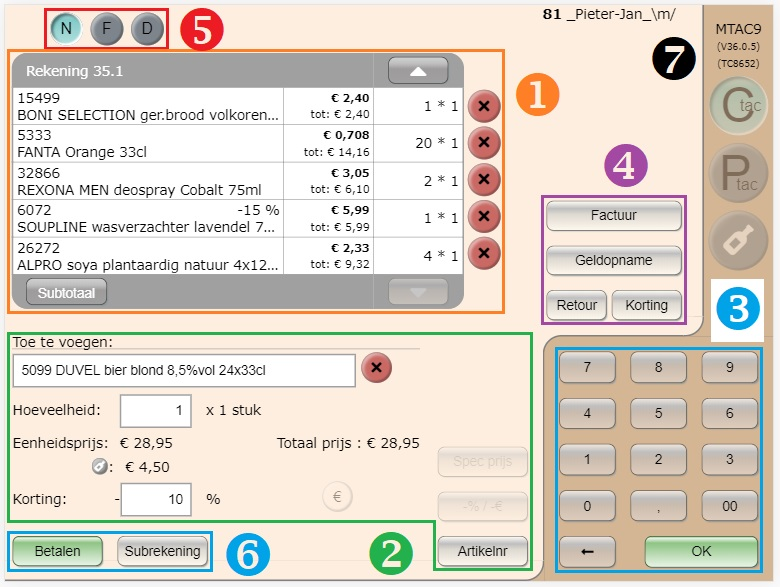
\includegraphics[scale=0.7]{img/func-omsch/CLP-CTAC-Aanduidingen.jpg}
    \caption{Basisscherm van het CTAC-gedeelte van de applicatie, met aanduiding van de verschillende onderdelen. \scriptsize Copyright~\copyright~Colruyt Group Services nv}
    \label{fig:Ctac-Aangeduid}
\end{figure}

\subsection{PTAC}

De verschillende componenten in het hoofdscherm van de PTAC opstelling worden in figuur \ref{fig:Ctac-Aangeduid} aangeduid. De belangrijkste componenten zijn:

\begin{figure}[h!]
    \centering
    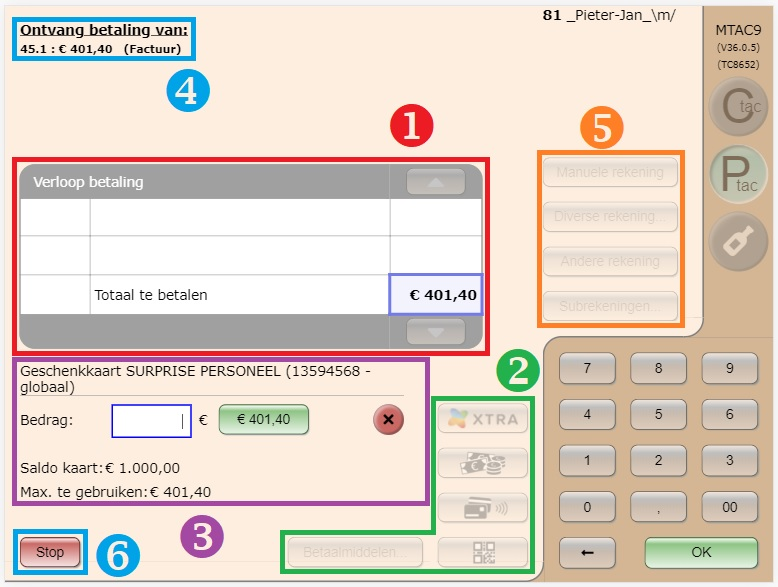
\includegraphics[scale=0.7]{img/func-omsch/CLP-PTAC-Aanduidingen.jpg}
    \caption{Basisscherm van het PTAC-gedeelte van de applicatie, met aanduiding van de verschillende onderdelen. \scriptsize Copyright~\copyright~Colruyt Group Services nv}
    \label{fig:Ptac-Aangeduid}
\end{figure}

\begin{enumerate}
    \item De \emph{CashMovementListComponent} \textbf{(1)} geeft een overzicht van de reeds uitgvoerde betalingstransacties alsook het totaal te betalen en het nog openstaande bedrag. Eenmaal de rekening volledig betaald werd, ziet men hier ook een eventuele geldteruggave of geldopname.
    \item De \emph{CashMovementButtonsComponent} \textbf{(2)} geeft de mogelijk betaalmiddelen weer. Men kan betalen met de betaalfunctie van de Xtrakaart of Colruytkaart, met cash, met een elektronisch betaalmiddel (bankkaart, maaltijdcheques etc.) of met MPAY. Minder gangbare betaalmiddelen zijn toegankelijk via de knop ``Betaalmiddelen...''.
    \item De \emph{CashComponent} \textbf{(3)} is beschikbaar eenmaal een betaalmiddel gekozen werd. Hier kan men het bedrag van de betaling bepalen — ofwel het saldo van de rekening, ofwel een manueel ingevoerd deel daarvan. Soms staat hier bijkomende informatie: figuur \ref{fig:Ptac-Aangeduid} toont een betaling met een geschenkkaart, die ook het saldo en het maximaal te gebruiken bedrag voor de betaling toont.
    \item De \emph{PaymentSubjectsOverviewComponent} \textbf{(4)} toont de te betalen rekening met hun totaal en eventueel relevante informatie — bijvoorbeeld als het gaat om een Factuur en/of als er een Xtra/Colruyt betaalkaart aangeboden werd voor de rekening.
    \item De \emph{SalesActionButtonsComponent} \textbf{(5)} is ook op de PTAC aanwezig en geeft een reeks opties met betrekking tot andere rekeneningen. Zo is het onder andere mogelijk om een andere (niet betaalde) rekening te openen ter betaling of, in het geval van subrekeningen, een rekening toe te voegen aan de betaling.
    \item De \emph{PaymentButtonsComponent} \textbf{(6)} bevat de knop die toelaat de betaling stop te zetten en de operator af te loggen op een PTAC opstelling. Op een MTAC opstelling laat deze knop toe terug te keren naar het artikelenoverzicht en krijgt de knop de benaming ``Terug''. Eenmaal een niet-omkeerbare betaling plaatsvond — bijvoorbeeld een betaling met de bankkaart — is deze knop uitgeschakeld.
\end{enumerate}